In the RL framework, there is a learner in a certain state $s$ and the learner executes an action $a$ to an environment based on her action policy $\pi^{(a)}$. Then, the environment gives a feedback in a form of a reward, $r$, and the learner updates her optimal policy $\pi^*$ in order to maximize her expected discounted future total reward: 
\[
	\mathbf{E}[r_t + \gamma r_{t+1} + \cdots + \gamma^{T-t}r_T | s_t, \pi^* ]
\]
where $T$ is time horizon and $\gamma$ is a discount factor which controls the relative importance of the immediate reward for the learner. If $\pi^{(a)}$ differs from $\pi^*$, the learning method is categorized to \textit{off-policy}, and if $\pi^{(a)} = \pi^*$, the method is \textit{on-policy}. In order to apply RL to a certain learning task, we need to define an appropriate learning system first. In this paper, we followed the learning system defined in \cite{Li}. 
\subsection{Learning System for Dialog Generation}
The learning system consists of two agents where they take turns talking with each other, $p_1, q_1, p_2, q_2, \cdots, p_t, q_t$. $p_i$ and $q_i$ represent $i$-th utterance of the first and the second agent in a conversation, respectively. Unlike the paper of \cite{Li}, we will use $u_i$ as a notation $i$-th utterance of a conversation regardless which agent spoke the utterance in order to make sure that the learning model is trained with both agents. \\
A state is defined by the previous two dialog turns, $s_t = [u_{t-1}, u_t]$. Specifically, the concatenated vector of the two utterance vectors is used as an input of the SEQ2SEQ encoder. An action $a$ is defined as a dialog utterance to generate. The action space, $\mathcal{A}$ is considered as an infinite space, but we constrained the maximum length of the generated utterance, $L$, and the number of available vocabularies, $|V|$ ($V$ is a set of available vocabulary). Therefore, $|\mathcal{A}|=L\times |V|$ in our model. The RL policy, $p_{RL}$ use the form of a SEQ2SEQ encoder-decoder defined by its parameters. 
\subsection{Reward}
\cite{Li} defined three reward functions and used the weighted sum of the rewards as a total reward. The first reward function measures the ease of answering a generated turn (or action) using the log likelihood of responding to that action with a dull response. They defined dull responses with 8 turns including "I don't know what you are talking about", "I have no idea", etc. The function is:
\begin{equation}
	r_{1,t} = -\frac{1}{N_{\mathcal{D}}} \sum_{d\in \mathcal{D}} \frac{1}{|d|} \log p_{seq2seq}(d|a_t)
\end{equation} 
where $\mathcal{D}$ is a set of dull responses and $p_{seq2seq}$ is a probability distribution with parameters learned by SEQ2SEQ. $p_{seq2seq}$ is different from $p_{RL}$. \\
The second reward function penalizes semantic similarity between consecutive turns from the same agent. They used cosine similarity to measure:
\begin{equation}
	r_{2,t} = -\log \cos (h_{u_{t-1}}, h_{a_t}) = -\log \cos \frac{h_{u_{t-1}}\cdot h_{a_t}}{||h_{u_{t-1}}||_2 ||h_{a_t}||_2} \label{eq:reward2}
\end{equation}
where $h_{u_{t}}$ is an SEQ2SEQ encoder output with the input $u_t$. \\
The last reward function addresses semantic coherence considering mutual information:
\begin{equation}
r_{3,t} = \frac{1}{|a_t|} \log p_{seq2seq} (a_t|u_{t-1},u_t) + \frac{1}{|u_t|} \log p_{seq2seq}^{backward}(u_t|a_t) \label{eq:reward3}
\end{equation}
where $ p_{seq2seq}^{backward}$ the probability distribution with parameters learned by SEQ2SEQ but with sources and targets swapped. Therefore, this backward SEQ2SEQ model has to be separately trained before using the RL rewards. 

\subsection{Model}
\begin{figure}[b!]
    \centering
    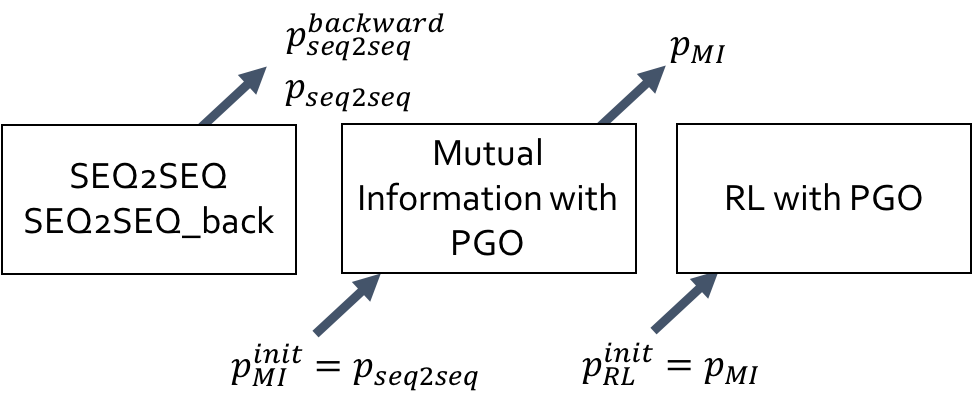
\includegraphics[width=0.4\textwidth]{three_steps.png} 
    \label{fig:three_steps}
    \caption{\small Training Procedure of the proposed Reinforcement Learning Model}
 \end{figure}
Any RL method falls into one of policy-based, value-based, or actor-critic RL areas. Among policy-based RL methods, a policy gradient optimization (PGO) using REINFORCE algorithm \cite{Williams} has been widely used. \cite{Li} also used the REINFORCE algorithm for learning the RL model. The training procedure of the RL model is divided into three steps as shown in the Fig.\ref{fig:three_steps}. First, we train a SEQ2SEQ model and a SEQ2SEQ backward model. Next, we train a mutual information model learned with PGO using the semantic coherence (Eq.\ref{eq:reward3}) as an only reward. As mentioned earlier, the two pre-trained models are used to compute the reward. The policy parameters of the model is initialized by the parameters of the pre-trained SEQ2SEQ model. The objective function to maximize is:
\begin{equation}
	J(\theta)= 	\mathbf{E} [m(\hat{a},[u_{t-1},u_t])]
\end{equation}
where $m(\hat{a},[u_{t-1},u_t])$ is equal to $r_{3,t}$ in the Eq.\ref{eq:reward3}. The gradient is estimated using the likelihood ratio trick in PGO:
\begin{equation}
	\nabla J(\theta) = m(\hat{a},[u_{t-1},u_t]) \nabla \log p_{RL}(\hat{a},[u_{t-1},u_t]) \label{eq:gradient}
\end{equation}

Then, we update the parameters in the encoder-decoder model using stochastic gradient descent (SGD). In addition to the standard PGO method, \cite{Li} adopted a curriculum learning strategy proposed by \cite{Ranzato} and a baseline strategy. The baseline strategy is common in implementing PGO method since PGO tends to have high variance, and the strategy helps to reduce the variance.
